\documentclass{article}
\usepackage{cgw}
\usepackage{epsf}
\usepackage{graphicx}
\usepackage{url}

\newcommand{\TODO}[1]{
\begingroup{\noindent\textbf{TODO:\ #1}}\endgroup%
}
\def\mmeta#1{\emph{$\cal MET\!\!A$#1$^2$}}

\title {Virtual Clusters as a New Service of MetaCentrum, the Czech NGI}
\author{Ruda, M.;
\v Sustr, Z.;
Sitera, J.;
Anto\v s, D.;
Hejtm\' anek, L.;
Holub, P.}

\institute{CESNET, z. s. p. o., Zikova 4, 160~00 Prague, Czech Republic}


\widowpenalty=10000
\clubpenalty=10000
\begin{document}
\maketitle

\begin{abstract}
MetaCentrum, the Czech NGI, started to virtualize the infrastructure several years ago.
%Major
%part of MetaCentrum computation resources is currently virtualized.
The virtual nature of the resources, being integrated with the resource management system, is mostly hidden to end users.
We are introducing a new public service ``virtual cluster'' which turns the virtualized infrastructure
into end user service. Virtual cluster service provides an illusion of totally dedicated clusters
running on a shared infrastructure under complete user control, including administrator access and
user specified application environment. Virtual machines and clusters are handled in a way similar to
ordinary computation jobs, planned for batch or interactive processing. We developed an extension to
job scheduler PBSPro and new management tools to smoothly integrate virtual cluster service into
production environment. Networking is a vital part of the service, where Czech NREN CESNET2
technology allows managing virtual cluster network without perceivable overhead. Virtual network
is seen as a new resource. 
%Benefits of this fully integrated virtualized infrastructure will be demonstrated through series of use cases.

\end{abstract}

\section{Introduction}

In recent years, virtualization of computing resources became one of key focal points of research and development
in MetaCentrum (\url{http://meta.cesnet.cz}). It allows applications with contradictory environment requirements to run on a single node, making it rather simple
to allocate resources available to each of them.

This year, MetaCentrum
introduces another step in development relying on the principles of virtualization---\emph{virtual clusters} enhanced with features
inspired by cloud computing, but oriented primarily on HPC user communities. The new solution allows users to request specific environment for their applications,
or even supply their own virtual images (appliances) to replace defaults made available by the service provider. Such images may be used to set up temporary
virtual clusters with a requested number of nodes, or to temporarily extend existing physical clusters with additional virtual nodes to handle peak loads.

The possibility to use custom images tuned to the needs of a specific application while setting up virtual clusters lowers the adoption threshold for potential new
users since the resulting virtual environment does not differ in any significant way from their current traditional environment.

\section{Architecture Overview}
\label{Architecture}

\begin{figure}[b]
\begin{center}
    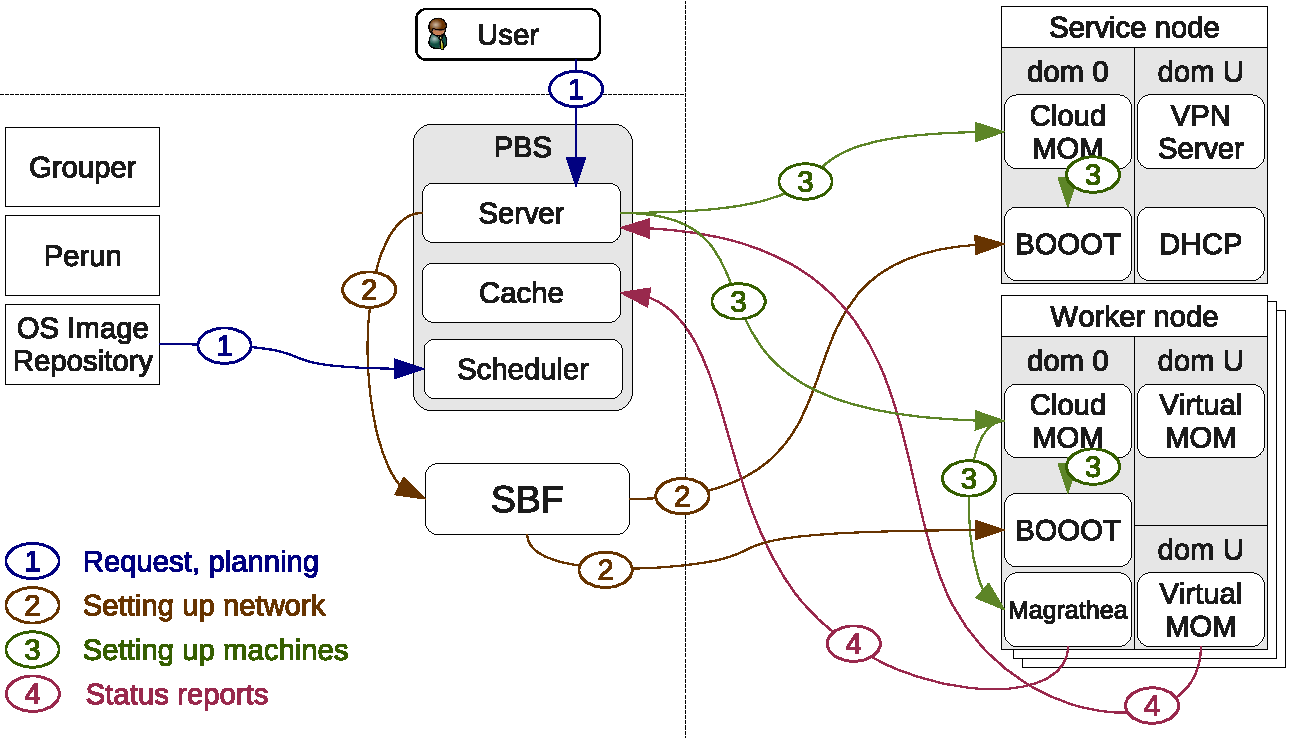
\includegraphics[width=.8\columnwidth]{cloud_arch.pdf}
\end{center}
    \caption{Overall architecture of the virtual clouds solution}
    \label{fig:architecture}
\end{figure}

Several services (Fig. \ref{fig:architecture}) had to be combined and adjusted to implement the functionality. Scheduling is done by MetaCentrum's PBSPro batch system, virtual image
handling and management is being carried out by Magrathea, virtual clusters are managed with SBF and virtual LANs interconnecting individual cluster nodes
rely on the advanced capabilities of the CESNET2 NREN.

PBS is the core service. It had to be modified to support new types of jobs (virtual clusters) and to communicate with Magrathea and SBF, requesting virtual machines and private networks as per user requirements. More extensions were required to implement authorization, allowing cluster owners to specify authorized users of their clusters by referencing system-wide groups.

Magrathea \cite{sc07} is an in-house developed system serving as an interface between the batch scheduling system and virtual machine monitors. It carries out
functions such as setting up, booting or terminating virtual machines, and provides essential feedback on the status or availability of physical
resources.

SBF is a tool used by the extended PBS to set up virtual networks~\cite{sbf}. 
The ability to insert custom virtual clusters into their separate virtual networks is vital from the security viewpoint. By allowing custom images, the service
provider relinquishes control of security within the cluster but encapsulates it in a private network to provide protection in both directions (protecting the
machines inside to allow the use of un-patched or outdated systems as required by users, while simultaneously protecting the outside world in case the virtual
cluster gets compromised), making the network accessible through a gateway and defining external resources accessible to machines within the network.

%Work presented here is a continuation of previous developments towards virtualization. Certain areas required only minor adjustments in this stage; others---such as PBS or Magrathea---were considerably extended and integrated to achieve the required functionality.


% Besides that, it is possible to suspend, preempt or even migrate
%virtual machines running long-term jobs, and create isolated environment to run legacy or special-purpose
%applications.

%\TODO{Dal bych sem nejake povidani, ze do vyreseni jsou zapojeny sluzby na kterych uz nejakou dobu
%delame (magrathea + rozsireni PBS, citace na sc07, SBF a virtualni site a citace na CGW08) a ze jsou v dalsich
%kapitolach jednotlive sluzby lehce popsany, rozepsana rozsireni pro nove vlastnosti... Ala Jirkovo
%Architecture:
%\begin{itemize}
%\item sem tu integraci, pov�d�n� jak jsme to meli nachystatn� a ted se to slozilo
%\item nejak� obr�zek, komponenty a jejich interakce (klidne ten co m�me)
%\item technicky popis co kter� komponenta celku dod�v�, klidne na pr�kladu vytvoren� clusteru
%\end{itemize}
%}

%We have created a system called Magrathea to allow job scheduling system to
%deal with several virtual machines running on a single computer and to submit
%jobs into those VMs.

\section{Magrathea---Scheduling Virtual Machines}
\label{magrathea}

The Magrathea System~\cite{sc07} has been developed to provide management of several virtual
machines running on a single computer and submit jobs to the proper ones.

Magrathea provides an interface between the batch scheduling system and virtual
machine monitors. It allows jobs to be submitted in a controlled manner into virtual
machines running on cluster nodes (with multiple virtual machines running on a single
cluster node). Magrathea can also be seen as a scheduler running on each cluster node,
scheduling virtual machines according to jobs submitted by batch scheduling systems.
Furthermore, Magrathea is designed to be independent on
a batch system and virtual machine monitors used on computational nodes,
current implementation supports  the PBSPro batch system
and Xen and VServer virtual machine monitors.

\subsection{Original Use Cases}
Development of Magrathea has been originally driven by three use cases:

\begin{description}
\item[Multiple static domains,] only one of them may run at any given time. 
Typically used for sharing nodes between mutually
incompatible projects. A single domain, running actual computational job, is assigned almost 
all available resources at a time, while the other domains are allowed to run with 
a minimum CPU and memory consumption,
just to appear available to their respective scheduling systems.

\item[High-priority jobs in privileged domains,]
%Jobs with higher priority 
such as interactive jobs required to run immediately, or massively parallel 
jobs whose processing would
be unfeasible should they have to wait until the full number of required processors is
actually free, may run in high-priority or ``privileged'' domains,
temporarily suppressing resources available to standard virtual domains. Jobs
in the standard domains are suspended, but still visible to
their respective scheduling and monitoring systems. This ensures that those
suspended jobs are not considered ``lost'' or aborted, and the
scheduler does not resubmit them to another node. The same technique of domain preemption
is used for giving cluster owners higher priority, while providing resources to rest 
of grid when cluster is not used.
\item [Suspending/freezing virtual machines] in order to run
services that only need to be available temporarily. Such machine or service can be 
suspended on demand, remain on ``stand-by'' and get reactivated quickly by service owner
when needed, instead of slow booting of all the nodes.
\end{description}

\subsection{Virtual Cluster Motivations}
Virtual clusters consist of virtual machines rather than actual physical ones,
abstracting from the physical topology of the underlying resources. This service
resembles, to certain extent, motivation for clouds ---virtual computing services
whose popularity has been growing in recent years.

Two additional use cases have been kept in mind while implementing functionality
required by virtual clusters:

\begin{description}

\item[Jobs running in an environment adjusted to their needs.] 
Jobs may require specific environment to run, installed for each job run separately 
from registered node images (appliances). Users may be allowed to
supply their own images, tuned specifically for compatibility with their applications.

\item[Virtual nodes used to form semi-permanent
virtual clusters] that may be only used for running specific
jobs, and consequently removed or kept back for future need. Jobs in such virtual
clusters may be managed either by central PBSPro installation provided by MetaCentrum
or may become an integral part of user's infrastructure,
subject to a common job and account management. With the latter approach, existing 
physical resources (clusters) may be
extended with additional virtual nodes, and physical or virtual nature of any given
node is completely transparent to the user.
\end{description}

\subsection{Architecture Extensions}

Several extensions to Magrathea implementation (for a full description of the architecture see~\cite{sc07})
were needed---support for user-supplied images and support for nodes without a running system.
In its original design, Magrathea process had to be installed inside each virtual machine, to allow 
easier management of booting and suspend/resume operations. Current implementation supports a special type 
of nodes, where the modification of user-supplied image is no longer required.

Largest changes to Magrathea system were required to support dynamic node installation, using an image specified in 
job description. Magrathea status of virtual machine (used by scheduling system, see section \ref{pbs}) was extended 
to support not only existing and running nodes, but also nodes which are not running, but can be potentially installed 
and booted. Current version of Magrathea supports complete management of VM life-cycle, including node preparation, 
boot and shutdown.

%\TODO{tenhle obrazek je sice hezky, ale zabere hrozne mista}
%\begin{figure}[tb]
%    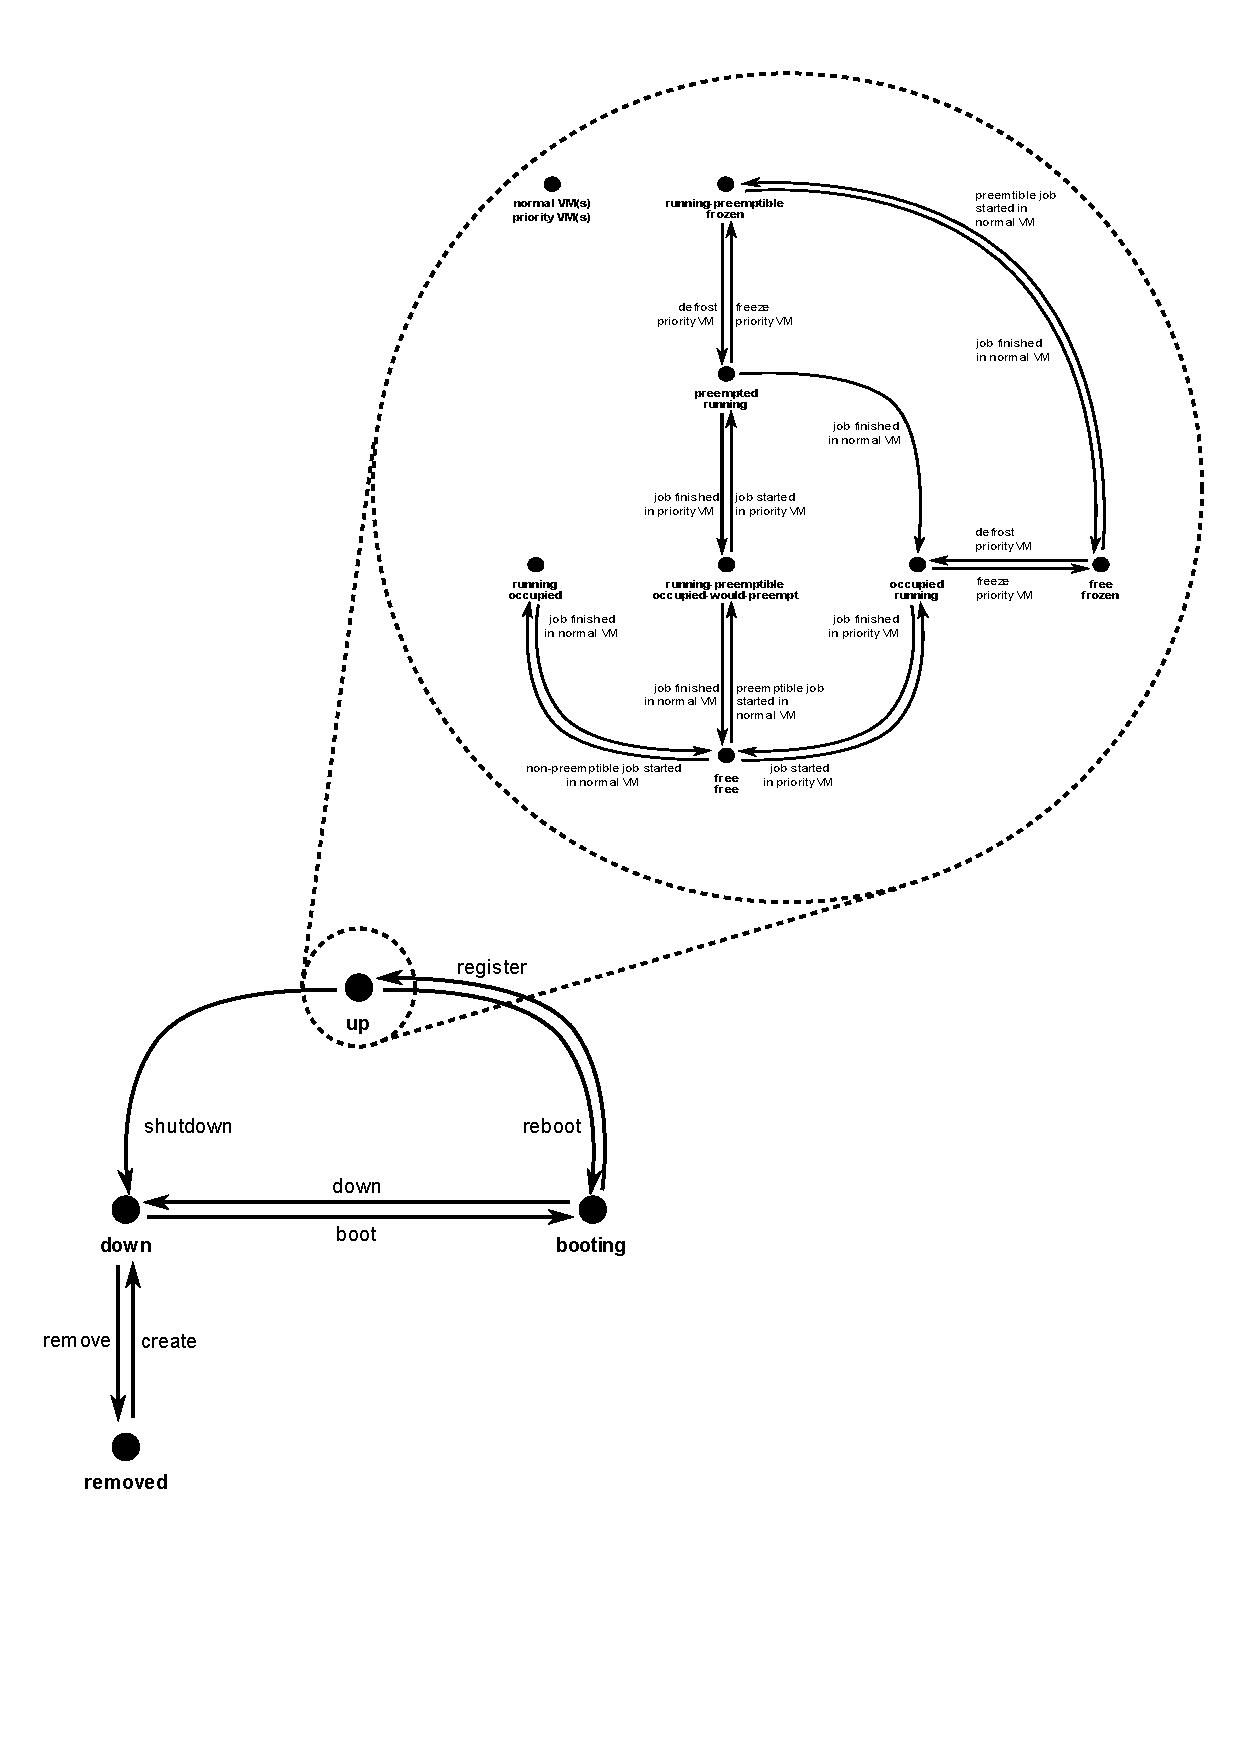
\includegraphics[width=.5\columnwidth]{lifecycle.pdf}
%    \caption{States and transitions between them}
%    \label{fig:lifecycle}
%\end{figure}

\subsection{Management of Virtual Images}

Management and deployment of virtual images is handled by Magrathea Booot module. 
It covers implementation of \textit{image repository}, which contains \textit{virtual appliances}~\cite{appliances}
(in the form of bootable images) together with metadata defining each appliance. The metadata contain
a description of the image is several senses:
\begin{description}
\item[image maintenance] -- image origin, owner, users allowed to use this image
\item[image requirements] -- on hardware (architecture, number of CPU, disk space)
\item[image properties] -- properties of the installed OS; used in standard batch systems for selection
 of needed functionality (OS flavor)
\end{description}
These metadata are used by the PBS Scheduler for matching possible nodes and images and for authorization decisions, and by deployment 
tools during the deployment phase.

\textit{Image deployment} tools support actual deployment of an image as well as configuration of the system within (network setup,
security keys assigned to this virtual image). Network setup is either static (predefined IPs and hostnames for virtual machines 
running ``certified'' images) or dynamic using DHCP.

\section{PBSPro Extensions}
\label{pbs}

PBSPro installation used in MetaCentrum was already modified~\cite{sc07} to support virtual machines managed by 
Magrathea. In a nutshell, the PBS Scheduler must take into account not only machine state
according to PBS, but also respect Magrathea status of virtual machines in the
process of selecting nodes for jobs. Using Magrathea status, scheduler 
can detect virtual nodes which are available as ``free'' in
PBS, but running on a physical node already occupied by another running virtual machine. 
For ``frozen'' domains, the PBSPro Server had to be also modified to handle cases of jobs running in a suspended domain.
The PBS must be aware of such a situation in order not to consider the machine and the job dead and to resubmit
the job to another machine.

Full support for virtual cluster management required wider modifications of PBSPro. 
PBS Scheduler supports nodes in ``down-bootable'' state, representing a situation where the node in not running, but the required 
image could be installed and started on this node. Such node can be selected to run jobs
even if the node is not usable according to PBS state (is not running). PBS Server was modified to handle such situations too; the request to start a virtual machine 
is redirected to a process running on the hosting domain---there, a slightly modified PBS Mom process is running and calling Magrathea services for 
VM management.

Virtual clusters are represented as a special type of job (cluster container) representing a submitted 
and/or running cluster. Scheduling such a container is 
similar to scheduling standard parallel jobs, with the exception of usability of potentially 
bootable nodes.
This approach unifies standard jobs and cluster containers for the scheduler.
Scheduler is using the same 
policy for all types of jobs, supports fair sharing of nodes between jobs and clusters. The implementation 
also fulfills another key requirement---ability to submit virtual clusters using standard PBS command 
line interface, with minimal difference to standard jobs. One new option \texttt{-l cluster} 
%\footnote{\texttt{-lcluster=[create,NAME][:group=GROUP][:net=private]}}
is supported by the \texttt{qsub} command used for job submission and image properties from metadata description of images can be used in node selection option 
\texttt{-lnodes}. 

%\TODO{jeste rict, ze do beziciho cluster se clovek dostava bud po svem nebo pomoci nasi PBS}
%Standard interfaces (PBS command line or
%web interface) may be used to submit jobs to these virtual clusters under common
%scheduling policies. 


\section{Networking}
The main motivation for incorporating the networking layer into virtual
cluster services is to hide the complexity of the underlying network
structure from the users. Every cluster, even spread over many sites
connected by nation-wide WAN network, can be seen as a single layer~2 network
segment. 

As described in section~\ref{Architecture}, separating the clusters
into discrete VLANs also encapsulates them in the sense of security.
The design and implementation of MetaCentrum virtual networks
is described in \cite{VirtCloud-CGW08, sbf}.
Virtual network management
(VLAN allocation service called SBF)
is integrated 
with the PBS-based virtual cluster manager.

In this paper, we discuss user access to the private virtual cluster
in case when the virtual cluster becomes a part of the
user's address space. IP addresses are configured by the user, the cluster is
connected to user's network by means of routing. 
The cluster falls completely into user's local network
policy and for the end user or anybody in the Internet it is not
distinguishable from a physical local cluster. This approach is suitable
for cases where departmental clusters exist
and we want to provide their administrators with tools allowing to use
MetaCentrum resources without adding any visible obstacles to the end users.

\begin{figure}[ht]
    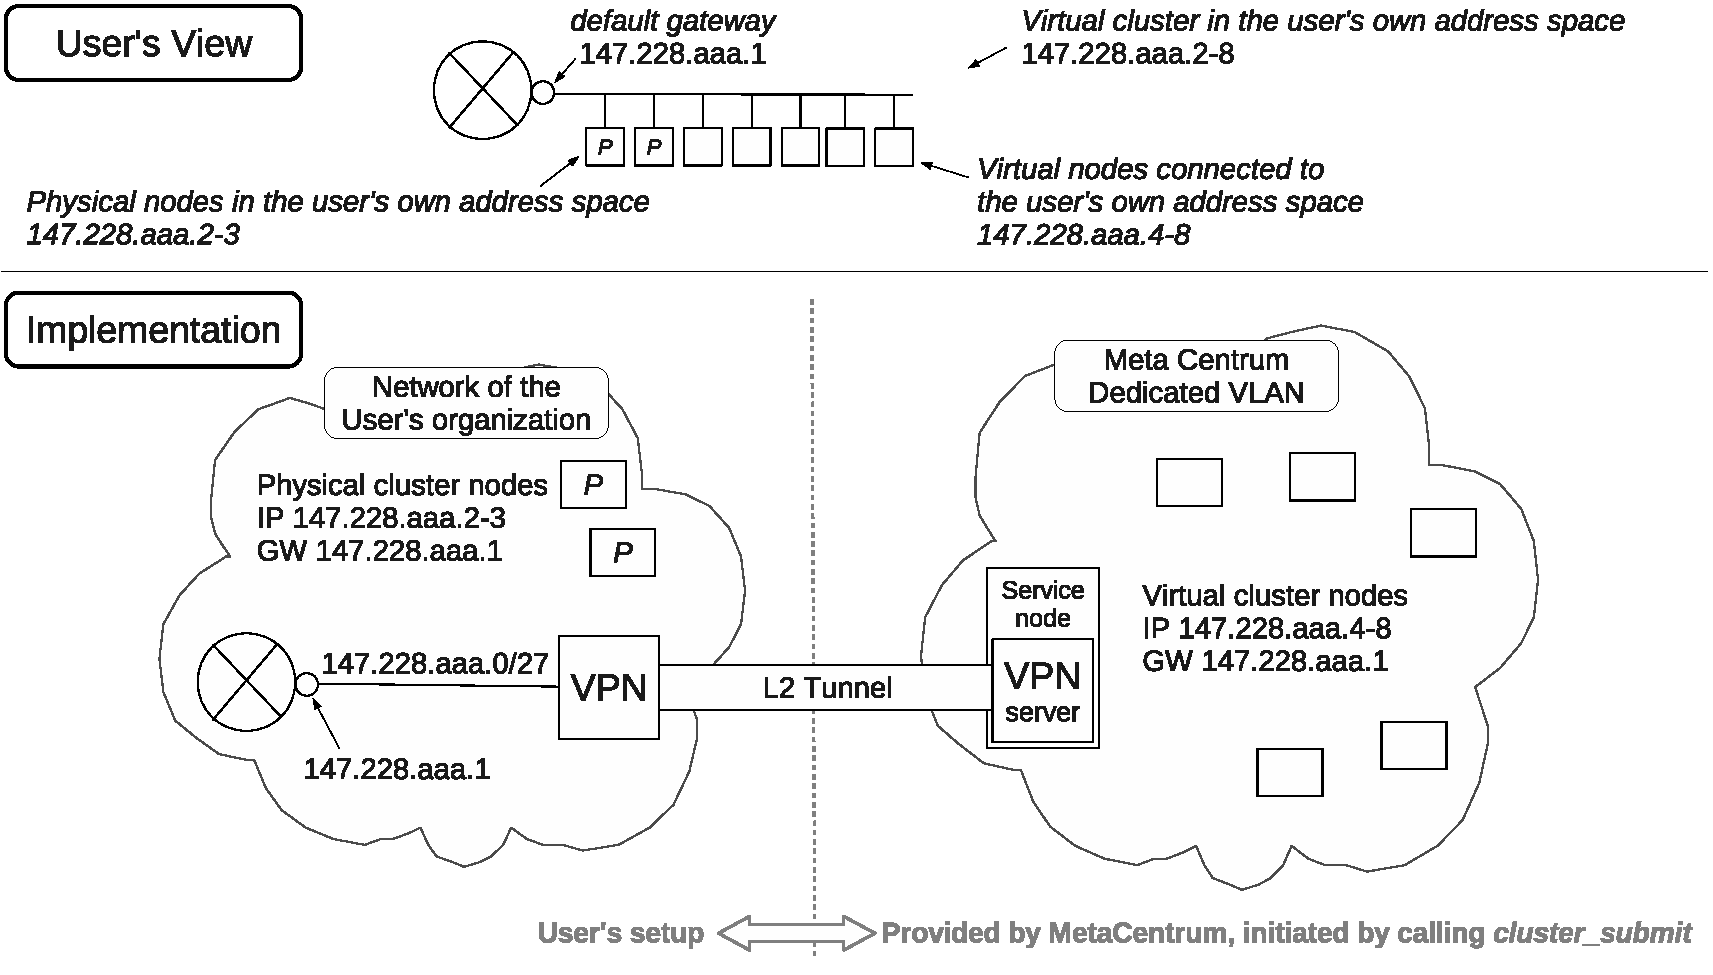
\includegraphics[width=\columnwidth]{publ.pdf}
    \caption{Virtual cluster publication as a part of user network}
    \label{fig:publication}
\end{figure}

Figure~\ref{fig:publication} shows the situation. The MetaCentrum virtual
cluster service consist of several virtual machines and one VLAN realized by  
advanced CESNET core network services (VPLS/Xponder
based). The VLAN is completely isolated at the MetaCentrum level and
the only connection to the outside network is realized on user
side. The tunnel is implemented by a VPN. In
MetaCentrum, the tunnel is ended by a service node of the virtual
cluster. That node is set up automatically by the virtual cluster management
services. The user side of the tunnel is implemented by a OpenVPN
client configured by the user. 
%We provide step-by-step instructions how to setup this software.

The virtual cluster management system includes support for IP address
assignment. The user provides the address block when submitting the
virtual cluster request and an automatically started DHCP
server on the cluster service node provides worker nodes of
the cluster with IP addresses.

%\section{Autorizace}
%
%\TODO{Co si troufneme slibit? Neni problem autorizace proti unixove grupe, zbytek bych asi dal do future work - reboot
%uzlu pres magratheu, uzivatelske grupy... mame neco do dalsiho clanku}
%
%\TODO{kde jsou popsany bezpecnostni problemy s cizim obrazem?}


\section{Related Work}

As virtualisation has recently become very popular in high performance
computing, several projects have emerged to deal with virtual machines
on worker nodes of computational clusters. As for the original motivation,
probably the closest project to ours is~\cite{karlsruhe}. Another interesting project aims to provide dynamic virtual
clustering~\cite{dvc} (DVC) using Xen virtual machine monitor, Moab workload
manager and Torque resource manager. Working in cooperation with Moab
developers the authors of DVC managed to provide transparent creation of
clusters of virtual machines. Virtual clusters are also allowed to span
multiple physical clusters by borrowing required resources from resource
managers of the other clusters. Integration of virtual machines to batch systems 
in EGEE project was motivation for work in \cite{irove}. Similar development 
was done in~\cite{cern}, where virtual machines are integrated with PANDA framework, using LSF batch system.

The idea of complete clusters of virtual machines, built on-demand and according to user specification, is 
one of the key features of clouds \cite{amazon}. Two open-source implementations of cloud technology \cite{workspaces,eucalyptus} 
can be referred as examples of cloud infrastructure, which allows user-supplied images of nodes to be started on
remote resources and arranged to sets of nodes comprising one group.

Management of virtual images was studied in \cite{appliances}, where a virtual appliance, as an application 
combined with an environment required by the application, was defined. Management and deployment of such images was 
studied for example in \cite{teragrid2007}, which also motivated our work. %Several pre-installed images 
%(including OSG and CernVM images) can be found in repository on \url{http://workspace.globus.org/vm/marketplace.html}.

Our work contributes to the world-wide effort by introducing characteristic cloud features into the HPC environment, and making them accessible---with minimal modifications---through traditional batch system interfaces. Integration with advanced networking services constitutes a complete solution for encapsulating virtual computing resources in virtual networks. Integration with cloud interfaces (Globus Workspaces) is going to continue into the future.

\section{Conclusion}

A prototype has already been deployed and the development has been catering for the needs of early adopters.
In foreseeable future, the solution will be made available across the whole National Grid Infrastructure and the development team will focus its efforts on its further evolution.

In the short term, the service will be extended with other features such as group authorization mechanisms, allowing owners to delegate permissions to handle (turn off, restart) their virtual clusters. Also, a virtual image repository service will be designed to handle standard images as well as custom images submitted by users.

Long-term goals include integration with cloud interfaces and extension of the system to support not only PBSPro but other batch job systems such as Torque as well.

\subsection*{Acknowledgments} 
%\begin{acknowledgement}
This work was done with the support of Ministry of Education of the Czech
Republic, research programs MSM0021622419 and MSM6383917201.
%\end{acknowledgement}

	\begin{thebibliography}{9}
	\bibitem{sc07} Ruda, M.; Denemark, J.; Matyska, L.: \emph{Scheduling Virtual Grids: the Magrathea System},
	   Second International Workshop on Virtualization Technology in Distributed Computing, USA,
	   ACM digital library, 2007. p. 1-7. 2007, Reno, USA.
	\bibitem{sbf}Anto\v s, D.; Matyska, L.; Holub, P.; Sitera, J.: \emph{VirtCloud: Virtualising Network
	   for Grid Environments-First Experiences}, The 23rd IEEE International Conference on Advanced
	   Information Networking and Applications AINA 2009. Bradford, UK : IEEE Comp. Soc., 2009. pp.
	   876-883, 8 p. ISBN 978-0-7695-3638-5
        \bibitem{VirtCloud-CGW08}
         Anto\v s, D., Sitera, J., Matyska, L., Holub, P.: \emph{MetaCenter
         Virtual Networks}. In Cracow Grid Workshop 2008. Cracow, Poland : Cyfronet
         AGH, Krak\'ow, Poland, 2009. pp. 86-93, 8 p. ISBN 9788361433002.
	\bibitem{karlsruhe}
	V. B\"uge, Y. Kemp, M. Kunze, O. Oberst, and G. Quast.
	\emph{Virtualizing a Batch Queuing System at a University Grid Center.}
	In {Frontiers of High Performance Computing and Networking -- ISPA
	Workshops}, Springer-Verlag LNCS 4331, 2006.
	\bibitem{dvc}
	W. Emeneker, D. Jackson, K. Butikofer, D. Stanzione.
	\emph{Dynamic Virtual Clustering with Xen and Moab}
	In {Frontiers of High Performance Computing and Networking -- ISPA
	Workshops}, Springer-Verlag LNCS 4331, 2006.
	\bibitem{workspaces}
	K. Keahey, K. Doering, and I. Foster. From Sandbox to Playground: \emph{Dynamic Virtual
	Environments in the Grid.} In: {5th International Workshop in Grid Computing
	(Grid 2004)}. 2004.
	\bibitem{cern}
	O. Khalid; Richard J. Anthony; P. Nilsson; K. Keahey; M. Schulz; K. Parrot; M. Petridis:
	\emph{Enabling and optimizing pilot jobs using xen based virtual machines for the HPC grid applications.} In
	VTDC '09: Workshop on Virtualization technologies in distributed computing,
	2009, Barcelona, Spain.
	\bibitem{irove}
	S. Childs, B. Coghlan, and J. McCandless. \emph{Dynamic virtual worker nodes in a production Grid.} 
        In Frontiers of High Performance Computing and Networking - ISPA
	2006 Workshops (XHPC 2006), volume 4331/2006, pages 417-426, Sorrento, Italy, December 2006.
	\bibitem{eucalyptus} Nurmi D., Wolski r., Grzegorczyk Ch., Obertelli G.,
	    Soman S., Youseff L., and Zagorodnov D. \emph{The eucalyptus
	    open-source cloud-computing system.} In Proceedings of Cloud
	    Computing and Its Applications, October 2008.
	\bibitem{teragrid2007}Bradshaw, R., N. Desai, T. Freeman, K. Keahey. 
        \emph{A Scalable Approach To Deploying And Managing Appliances.}TeraGrid 2007, Madison, WI. June
	2007.
	\bibitem{appliances} Sapuntzakis C., Brumley D., Chandra R., Zeldovich N., Chow J., Lam M. S., and Rosenblum M..
	\emph{Virtual Appliances for Deploying and Maintaining Software.}
	In Proceedings of the Seventeenth Large Installation Systems Administration Conference (LISA 2003), San Diego, CA, pages 181-194, October 2003.
	\bibitem{amazon}Amazon Web Services. Amazon Elastic Compute Cloud (ec2). \url{http://aws.amazon.com/ec2}
	\end{thebibliography}

\end{document} 
